\section{GTFS}
\label{sec:gtfs}

The adoption of GTFS \citep{GoogleDevelopers_2006} to public transport agencies around the world has made it possible for apps such as Google Maps to access and display public transport data to users, regardless of their location. The main goal of GTFS is to specify, in detail, how transit data should be organised so that it is consistent across agencies around the world. Whether you are in Auckland, Paris, or C\'ordoba, Google Maps is able to show you public transport directions because their transit data are defined using the same standard.


\GTFS{} consists of two components, \emph{static} and \emph{\rt{}}. The static component specifies how information portaining to the schedule, fares, and route geography are organised, while the \emph{\rt{}} component specifies the format for \rt{} data: vehicle locations, stop updates and \glspl{eta}, and service advisories. Each of the static and \rt{} components are implemented by a transit provider; for example \AT{}'s \GTFS{} service is hosted at \url{https://dev-portal.at.govt.nz}.


\subsection{Static GTFS}
\label{sec:gtfs_static}


\begin{table}[t]
\centering
\begin{tabular}{ll}
\toprule
Term & Definition \\
\midrule
route & a collection of \emph{trips} that are displayed to comuters
as a single service \\
trip & a journey servicing two or more stops at a specific time \\
stop & a location where passengers are picked up or dropped off \\
stop time & the (scheduled) times at which vehicles
will arrive at stops for each trip \\
shape & the GPS track a vehicle will take for a specific route \\
\bottomrule
\end{tabular}
\caption{Definitions of relevant GTFS terms, taken from\\
\url{https://developers.google.com/transit/gtfs/reference/}}
\label{tab:gtfs_terms}
\end{table}


There are several components of GTFS that are of particular interest to us: routes, trips, stops, stop times, and shapes. The definitions of these terms are given in \cref{tab:gtfs_terms}. Extensive documentation can be found on these and the other components on the GTFS website (\url{https://developers.google.com/transit/gtfs/}) \citep{GoogleDevelopers_2006}.


\Cref{fig:gtfs_nw} demonstrates a single \emph{route}, along which there are two active \emph{trips} (A and B). The route's \emph{shape} is represented by the line connecting the six \emph{stops} numbered 1--6. The \rt{} arrivals board is shown for stop~5, displaying the scheduled \emph{stop time} (arrival time) for each trip at that stop. The additional information displayed is described in the next section.



\begin{knitrout}\small
\definecolor{shadecolor}{rgb}{0.969, 0.969, 0.969}\color{fgcolor}\begin{figure}

{\centering 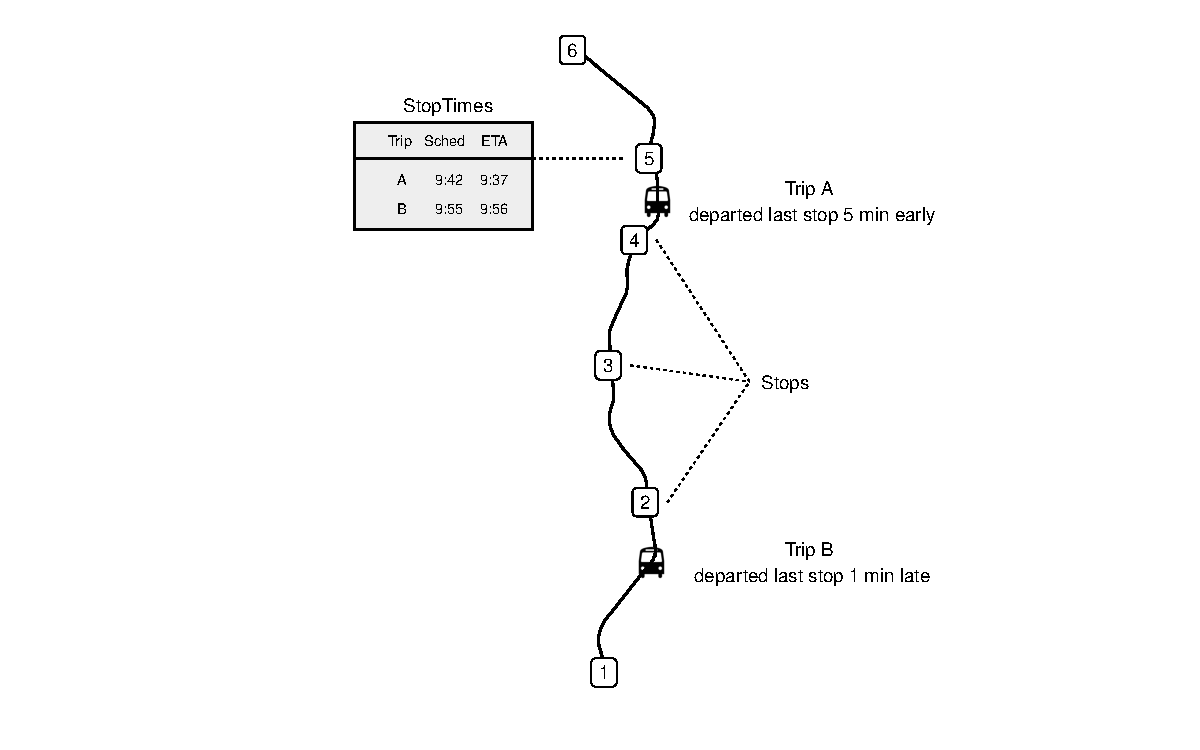
\includegraphics[width=\textwidth]{figure/gtfs_nw-1} 

}

\caption{A \gls{gtfs} diagram of a single \emph{route}, showing two \emph{trips} (A and B) travelling along the route's \emph{shape} path. The numbered squares represents \emph{stops}, and the scheduled arrival times of each trip at stop 5 are displayed in the \emph{stop times} box.}\label{fig:gtfs_nw}
\end{figure}


\end{knitrout}



Static \GTFS{} data is typically distributed by transport providers as plain text files, one for each of the components (such as \verb+routes.csv+ and \verb+trips.csv+). Often these are available to download as a single ZIP archive, so the data can easily be loaded into a \emph{relational database}. \Cref{app:gtfs} describes the relational structure of the \GTFS{} database. The R package developed as part of this work provides the \verb+create_gtfs()+ function to do this automatically:
\begin{knitrout}\small
\definecolor{shadecolor}{rgb}{1, 1, 1}\color{fgcolor}\begin{kframe}
\begin{alltt}
\hlkwd{library}\hlstd{(transitr)}
\hlstd{nw} \hlkwb{<-} \hlkwd{create_gtfs}\hlstd{(}\hlstr{"at_gtfs.zip"}\hlstd{,} \hlkwc{db} \hlstd{=} \hlstr{"at_gtfs.sqlite"}\hlstd{)}
\end{alltt}
\end{kframe}
\end{knitrout}




Within these separate files or tables, the data is stored as per \GTFS{}. Importantly, shapes are stored as sequences of coordinates that draw a path on a map, while stops are represented as a single coordinate marking the location of the bus stop. Stop times are stored in trip-stop pairs\footnote{It is a pivot table, if you know what that is.}, with one row for every stop of each trip, along with the scheduled arrival and departure times\footnote{There are 732,184 rows in the stop times table for Auckland Transport!}.



On its own, the static \GTFS{} information is as useful as a printed timetable, allowing simple journey planning to take place. It therefore provides the necessary ``fallback'' state in cases where no \rt{} information is available for a given trip. In later sections, scheduled stop times are used to obtain \emph{prior information}, a core component of the Bayesian paradigm.



\subsection{\Rt{} GTFS}
\label{sec:gtfs_rt}

The \rt{} component of \GTFS{} is responsible for handling vehicle positions, trip updates (arrivals and departures from stops), and service alerts (cancellations and stop closures, for example). Data is processed by a central server, and then stored in an appropriate fashion to enable quick access via \glspl{api}. There is therefore the additional need of a server that can handle vast numbers of \gls{api} requests, meaning only a subset of the transport providers using \GTFS{} have also implemented the \rt{} component. Below we give a brief summary of these components, but further information can be read on the \GTFS{} website\footnote{see \url{https://developers.google.com/transit/gtfs-realtime/}.}.


\subsubsection{Vehicle positions}
\label{sec:gtfs_rt_vehicle}

The key components of a vehicle position (in the context of \GTFS{}) are a \emph{vehicle descriptor} which includes information about the physical vehicle, a \emph{trip descriptor} which holds information about the trip being serviced, a \emph{timestamp} specifying exactly when the observation was made, and a \emph{position} containing the actual data, such as the \gls{gps} observation.

The specification also allows for additional measurements, such as \emph{speed} or an \emph{odometer} reading. However, these were not available from \AT{} at the time this work was carried out, so we have not included them in our framework. It is well worth noting, however, that they could be integrated with minimal effort if they become available.


\subsubsection{Trip updates}
\label{sec:gtfs_rt_trip}

As vehicles equipped with \gls{avl} technology arrive at and depart from stops, information about their time of arrival, and most importantly \emph{schedule adherence}, is stored in trip updates. These also contain a \emph{trip descriptor}, as well as one or more \emph{stop time updates}. \AT{} provides a single stop time update for the most recently visited stop; however, it is possible to retain all previous stop time updates, as well as provide predictions for upcoming stops.


Each stop time update reports either the arrival or departure time and, where schedule information is available, the schedule adherance by way of an \emph{arrival} or \emph{departure delay} (in seconds). The onboard \gls{avl} device is responsible for detecting these events, and they are not necessarily linked to the \gls{gps} position of the vehicle. In Auckland, each trip update also triggers a vehicle location update, but the coordinates are those of the \emph{stop} and not the vehicle, which can cause problems we address in \cref{sec:realtime-data}.



\subsubsection{Service alerts}
\label{sec:gtfs_rt_alerts}

Less important for the current work, but essential for reliable \gls{rti}, \emph{service alerts} enable transit operators to modify the static \GTFS{} in \rt{}. So, when a trip is cancelled, they have the ability to send out a service alert announcing the cancellation\footnote{Although they often don't.}. This is often displayed to passengers as a ``C'' on the \rt{} board. It is also possible to add trips, for example during special events, or to reroute trips around stop closures, but this is beyond the scope of our work.



\subsection{Accessing \rt{} data (API)}
\label{sec:gtfs_rt_api}

In order to distribute vehicle locations, trip updates, and service alerts to passengers quickly and usefully requires more than just a \rt{} board at bus stops. Personal mobile devices have revolutionised the way we live our lives, and developers are constantly creating new apps to assist with everyday activities. Included in these are transit apps, which are capable of passing on \rt{} \GTFS{} data to passengers.

The most common method of distributing \rt{} data is via an \gls{api}. These are, in simple terms, a fixed web address from which developers can request a data file---either JSON or, in the case of some \GTFS{} systems, protobuf \citep{cn}---which can then be parsed and displayed to users. Usually developers need to register for an \emph{\gls{api} key} which helps to control server demand by limiting the number of requests a user can make, or controlled access to specific data. Our R package includes the ability to connect to a \GTFS{}-based \gls{api} easily using the following command:
\begin{knitrout}\small
\definecolor{shadecolor}{rgb}{1, 1, 1}\color{fgcolor}\begin{kframe}
\begin{alltt}
\hlstd{url} \hlkwb{<-} \hlstr{"https://api.at.govt.nz/v2/public/realtime/vehiclelocations"}
\hlstd{nw} \hlkwb{<-} \hlkwd{load_gtfs}\hlstd{(}\hlstr{"at_gtfs.sqlite"}\hlstd{)} \hlopt
    \hlkwd{realtime_feed}\hlstd{(url)} \hlopt
    \hlkwd{with_headers}\hlstd{(}
        \hlstr{"Ocp-Apim-Subscription-Key"} \hlstd{=} \hlkwd{Sys.getenv}\hlstd{(}\hlstr{'APIKEY'}\hlstd{)}
    \hlstd{)}
\end{alltt}
\end{kframe}
\end{knitrout}
